%********************************************************************
% Appendix
%*******************************************************
% If problems with the headers: get headings in appendix etc. right
%\markboth{\spacedlowsmallcaps{Appendix}}{\spacedlowsmallcaps{Appendix}}
\chapter{Superficies brillosas}\label{ch:appendixSpecularSurfacesProblems}

En la \autoref{fig:ejemploProblemaMedicionSuperficieBrillosa} se puede observar un ejemplo de las limitaciones del dispositivo. Este ejemplo corresponde a un sector de la medición del \autoref{ch:appendixSampleScanImages}. La superficie real del objeto no tenía ningun defecto ni discontinudad en la sección observada. Sin embargo las reflexiones causadas por la superficie brillosa hacen que la decodificación de los patrones sea incorrecta.

\begin{figure}[!bth]
    \myfloatalign
        \subfloat{
            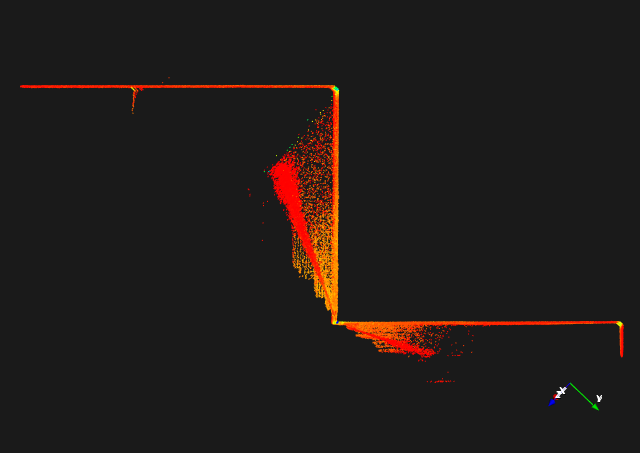
\includegraphics[width=0.49\linewidth]{images/soft/reflectionProblem3dView4}
        }
        \subfloat{
            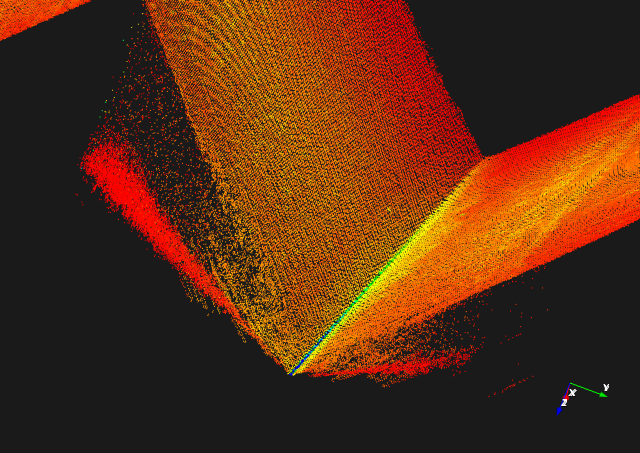
\includegraphics[width=0.49\linewidth]{images/soft/reflectionProblem3dView2}
        }
        \\
        \subfloat{
            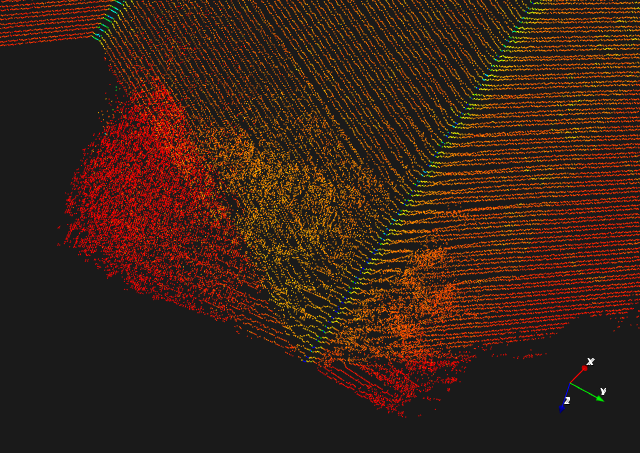
\includegraphics[width=0.49\linewidth]{images/soft/reflectionProblem3dView3}
        }
        \subfloat{
            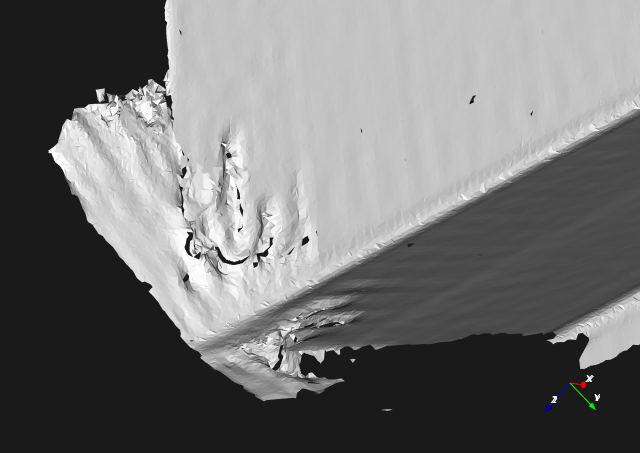
\includegraphics[width=0.49\linewidth]{images/soft/reflectionProblem3dViewSurface1}
        }
        \caption{Ejemplo de un problema causado por superficie brillosa}
        \label{fig:ejemploProblemaMedicionSuperficieBrillosa}
\end{figure}

En la \autoref{fig:ejemploCausaProblemaMedicionSuperficieBrillosa} se puede observar en detalle la sección de las imágenes donde se produce el problema. Queda claro que el reflejo de la superficie inferior sobre la superior es observado como un patrón fantasma/incorrecto, y lo mismo ocurre en la otra dirección (reflejo de la superficie superior sobre la inferior). Esto se debe a la combinación de la superficie brillosa junto con la dirección del eje de observación (ubicación de la cámara), la inclinación de las superficies de la pieza y la dirección de incidencia de la luz (ubicación del proyector). 

Este inconveniente no es observado en las imágenes correspondientes a la otra cámara, debido a que se forma otro ángulo entre la superficie, el proyector y la cámara, lo cual reduce considerablemente la magnitud del reflejo. 

\begin{figure}[!bth]
    \myfloatalign
        \subfloat{
            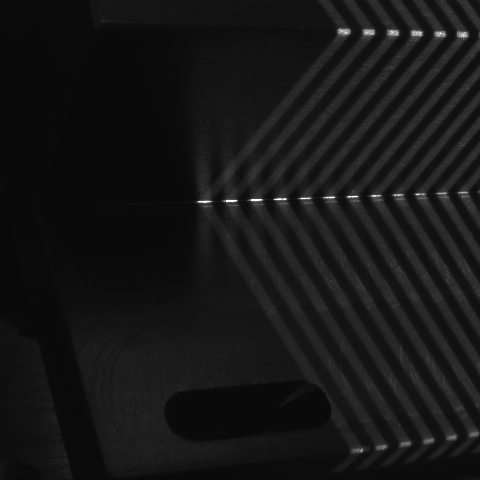
\includegraphics[width=0.49\linewidth]{images/soft/reflectionProblemCause1}
        }
        \subfloat{
            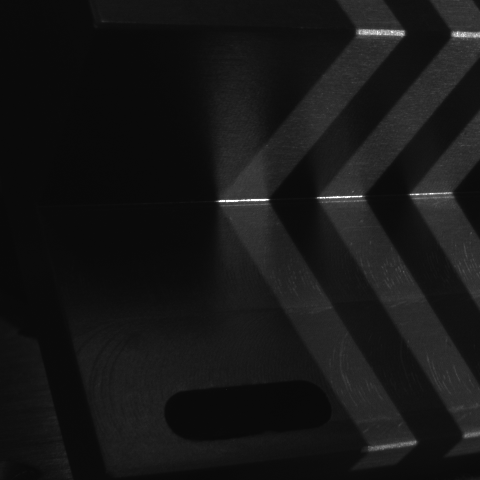
\includegraphics[width=0.49\linewidth]{images/soft/reflectionProblemCause2}
        }
        \caption{Causas de la decodificación incorrecta}
        \label{fig:ejemploCausaProblemaMedicionSuperficieBrillosa}
\end{figure}

En este caso la solución es simple, simplemente se busca una ubicación en la cual este inconveniente no afecte a ninguna de las cámaras. En el caso de que la superficie sea muy brillosa, muy oscura o transparente, se puede utilizar una capa muy fina de talco/polvo. Se pueden comprar aerosoles especialmente diseñados que cubren la superficie con una capa muy fina de polvo, logrando obtener una apariencia mate y de un color claro. Estos aerosoles contienen una suspensión de partículas blancas en un solvente de secado rápido. Un ejemplo\footnote{\url{https://ssl.david-vision-systems.de/shop/product_info.php/info/p105_3D-Coating-Spray.html}} se puede ver en la \autoref{fig:david3DcoatingSpray}.

\begin{figure}[!bth]
    \myfloatalign
        \subfloat{
            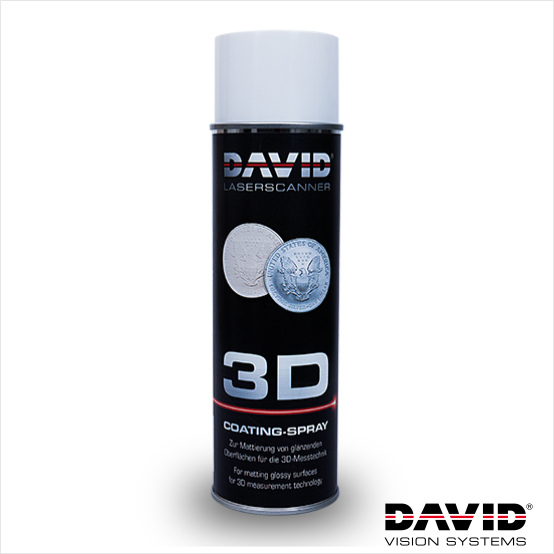
\includegraphics[width=0.49\linewidth]{images/david-3d.com/COATING-SPRAY-500}
        }
        \caption{Spray para la medición de superficies brillosas}
        \label{fig:david3DcoatingSpray}
\end{figure}